\documentclass{article}

\usepackage{epigraph}
\usepackage{graphics}
\usepackage{graphicx}
\usepackage{float}
\usepackage{amsmath}
\usepackage{listings}

\usepackage{epigraph}

\title{\textbf{ CS699 LaTeX Advanced Lab}}
\author{ Hareesh }

\begin{document}

\maketitle
\newpage

\tableofcontents
\newpage


\section{Introduction}
\subsection{Preface}

\hspace{1cm} As we all know that water gives life to us and other living things on the earth. It is very essential to continue life on the earth and other planets. Without water, we cannot imagine the existence of life on any planet. Earth is the only known planet having water and life till date. So, we should not ignore the importance of water in our life and try our best to save water using every possible means. The earth is covered with around 71\% water however with less amount of drinking water. The normal cycle of water balance runs naturally like evaporation and raining. However, the problem is with the saving of safe and drinking on the earth which is available in very less amount. Water conservation is possible with the good habits of the human beings.

\subsection{Why we should Save Water}
\hspace{1cm}In order to know the answer of why we should save water, first we should know the importance of water means how the water is valuable to us in our life. Life is not possible without oxygen, water and food. But most importantly water is most precious in all the three essentials of life. The question is how much pure water we have on the earth.\\
\hspace{1cm}According to the statistics, it has been estimated that less than 1\% of the water on the earth is suitable for drinking. If we estimate the ratio of drinking water and total population of the world, it would be, more than a billion of people all across the world are surviving on 1 gallon of water per day. It has also been estimated that around or more than 3 billion of people would suffer water shortages by 2025.
\subsection{Matrix}
\subsection{Matrix}

\section{Mathematical formulas and notations} %DO NOT CHANGE
\subsection{Matrix}
Adjacency matrix of corresponding graph.


\begin{table}[H]
\centering
\begin{tabular} {l | l}

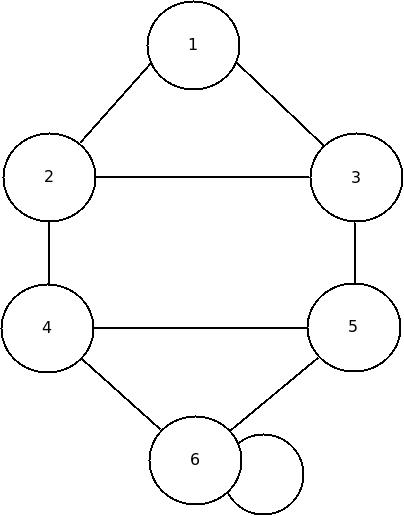
\includegraphics[width=6cm,height=3.5cm]{flow.jpeg}
   & 
ds

 \\

\end{tabular}
\end{table}



\subsection{Equation array}
\[cos 2\theta=\cos^2\theta-\sin^2\theta\]
\[=2\cos^2\theta-1\]


\[\cos^3\theta+\sin^3=(\cos\theta+\sin\theta)(\cos2\theta−\cos\theta\sin\theta)\]
\[=(\cos\theta+\sin\theta)(1−\cos\theta\sin\theta)\]
\[=\cos\theta+\sin\theta)(1/2)(2−2\cos\theta\sin\theta)\]
\[=(1/2)(\cos\theta+\sin\theta)(2−\sin(2\theta)\]
\\


\subsection{Prepositional formulae using various operators}
$\neg(\forall x)(\varphi(x)) \longleftrightarrow (\exists x)\neg\varphi(x)$ \\
$(\forall x)(\varphi(x)\Lambda\psi(x)) \longleftrightarrow ((\forall x)\varphi(x)\Lambda(\forall x)\varphi(x))$ \\
$(\exists x)(\varphi(x)\Lambda\psi(x)) \longleftrightarrow ((\exists x)\varphi(x)\Lambda(\exists x)\psi(x))$\\
$((\forall x)\varphi(x)\Lambda(\forall x)\psi(x)) \longrightarrow (\forall x)(\varphi(x)\Lambda\psi(x))$\\
$(\exists x)(\varphi(x)\Lambda\psi(x)) \longrightarrow  ((\exists x)\varphi(x)\Lambda(\exists x)\varphi(x)\Lambda(\exists x)\psi(x))$\\
\\


\subsection{Alphabets}

\begin{table}[H]
\centering
\begin{tabular} {| l | c |}
\hline
Greek letters: &
$\alpha  A  \beta  B \gamma \Gamma \rho \varrho P  \sigma \Sigma  \delta \Delta \epsilon  \varepsilon  E $\\
\hline
Binary operators: &
$\times \otimes \oplus \cup \cap$ \\
\hline
Relation operators:&
$\subset \supset \subseteq \supseteq < >  $\\
\hline
Others:&
$\int \oint \sum \prod$\\
\hline
\end{tabular}
\end{table}


\subsection{Mathematical Formulas}

\section{Mathematical formulas and notations}
\subsection{Matrix}
\subsection{Matrix}
\subsection{Matrix}
\subsection{Matrix}

\section{Algorithm and Pseudo code} %DO NOT CHANGE
\subsection{Tabbing}
 \lstinputlisting{bfs.cpp}

\subsection{Listing}

 \lstinputlisting[language=c]{bfs.cpp}
\subsection{Verbatim}
\begin{verbatim}
 //Breadth First Search Function
void BFS(list<longlong int> queue,long long int length){
	long long int v;
	if(queue.empty())
		return;
	list<long long int>::iterator i;
	list<long long int> queue temp;
	while(!queue.empty()){
		v=queue.front();
		queue.pop front();
		for(i=adj[v].begin();i!=adj[v].end();i++){
			if(!pro ver[*i]){
				result[*i]=length;
				queue temp.push back(*i);
				pro ver[*i]=true;
				adj[*i].remove(v);
			}
		}
	}
	BFS(queue temp,length+6);
}
\end{verbatim}

\subsection{Algorithmic}



\section{Tree} %DO NOT CHANGE

\section{Mathematical formulas and notations}
\subsection{Matrix}
\subsection{Matrix}
\subsection{Matrix}
\subsection{Matrix}

\section{Mathematical formulas and notations}

\epigraph{All human things are subject to decay, and when fate 
summons, Monarchs must obey}{\textit{Mac Flecknoe \\ John Dryden}}
 
\subsection{Matrix}
\subsection{Matrix}
\subsection{Matrix}
\subsection{Matrix}

\section{Bibliography}
\begin{thebibliography}{9}
\bibitem{Firuza Aibara} 
Firuza Aibara. LaTeX - Fundamental Research Group - IIT Bombay.
http://www.it.iitb.ac.in/frg/wiki/index.php/LaTeX/, 2016
 
\bibitem{Michael Downe} 
Michael Downes. \textit{Short math guide for LATEX}. American Mathematical
Society, 2002..
 
\bibitem{ Helmut Kopka} 
 Helmut Kopka and Patrick W Daly. A guide to latex, 1995.
 
\bibitem{Leslie Lamport} 
Leslie Lamport. \textit{Latex}. Addison-Wesley, 1994.
\end{thebibliography}

\end{document}